\chapter{ Distribuição dos Tópicos obtidos pelos extratores}\label{apendice3}




Nesse apêndice podem ser observadas as distribuições dos tópicos obtidos pelos extratores.
Os extratores K-Means, LDA e PLSA foram executados com o \textit{corpus} estudado nesse trabalho, do qual extraiu-se 70 tópicos com 5 descritores por tópico. Os tópicos extraídos são representados por seus descritores e as colunas marcadas com \#Seg indicam a quantidade de segmentos atribuída a um tópico.
Os dados podem ajudar a entender a distribuição dos assuntos registrados na coleção de documentos, conforme discutido no Capítulo~\ref{cap3}.

\begin{landscape}% Landscape page

	% 
\begin{table}[!h]
	\tiny
	\centering
	\begin{tabular}{|l|c||l|c||l|c|} 
		\hline


		\multicolumn{2}{|c||}{ \textbf{K-Means} } & \multicolumn{2}{c||}{ \textbf{LDA} } & \multicolumn{2}{c|}{ \textbf{PLSA} } \\ \hline
		\textit{Descritores} & \textit{\#Seg} & \textit{Descritores} & \textit{\#Seg} & \textit{Descritores} & \textit{\#Seg} \\ \hline



   dia; realizada; chamada; estado; conselho;    &   116  &         disciplinas; cursadas; fichas; caracterização; aprovado;    &   107  &       docentes; presidente; dia; discente; téc;    &   76   \\ \hline
   informado; compra; ofício; pedido; processo;    &   106  &         colocar; deve; poderia; referentes; seriam;    &   94  &       disciplinas; álgebra; linear; geometria; analítica;    &   75  \\ \hline
   computação; conselho; aprovado; acordo; ficou;    &   102  &         docentes; presidente; técnica; dia; administrativo;    &   91  &       computação; acordo; levada; chefia; conselho;    &   62  \\ \hline
   docentes; técnica; administrativo; presidente; dia;    &   72  &         dia; aprovado; aprovação; ordem; anterior;    &   85  &       aprovado; aprovação; unanimidade; foram; ordinária;    &   57  \\ \hline
   representante; discente; presidente; secretária; turma;    &   55  &         representante; técnica; administrativo; secretária; discente;    &   79  &       representante; discente; piccoli; turma; pauta;    &   51  \\ \hline
   cursadas; conselho; coordenação; computação; presidente;    &   45  &         conselho; junto; assina; acordo; ficou;    &   69  &       técnica; administrativo; representante; secretária; discente;    &   45  \\ \hline
   aprovado; aprovação; atividades; relatórios; lido;    &   44  &         seguintes; chamada; conselho; data; ano;    &   67  &       comunicação; presidência; informado; verba; ocorrerá;    &   38  \\ \hline
   computação; cursadas; conselho; título; discente;    &   37  &         presença; realizada; cidade; leme; métricas;    &   55  &       bacharelado; coordenação; cursadas; encerrada; acordo;    &   37  \\ \hline
   disciplinas; cursadas; libras; conselho; aprovado;    &   36  &         presidência; comunicação; informado; iniciou; agradeceu;    &   54  &       afastamento; aprovado; aprovação; apresentar; referentes;    &   35  \\ \hline
   professores; colocar; regras; seriam; sugeriu;    &   30  &         atividades; extensão; relatórios; aprovado; aprovação;    &   52  &       dia; ordem; anterior; informado; pedido;    &   35  \\ \hline
   pedido; informado; substituí; laboratório; disciplinas;    &   30  &         havendo; lavra; iniciou; trabalho; trata;    &   46  &       discente; representante; lúcio; presidente; seki;    &   34  \\ \hline
   aprovado; trocar; pedido; analisada; fichas;    &   28  &         verba; compra; pagamento; valor; material;    &   46  &       informado; compra; ofício; material; verba;    &   34  \\ \hline
   dia; ordem; concurso; dezembro; foram;    &   27  &         afastamento; aprovado; aprovação; relatórios; lido;    &   44  &       presidente; presentes; lavra; havendo; comunicou;    &   30  \\ \hline
   representante; administrativo; técnica; discente; secretário;    &   26  &         coordenação; deliberar; restrito; junto; assina;    &   39  &       dia; seguintes; presidente; realizada; participante;    &   28  \\ \hline
   afastamento; aprovado; referentes; relatórios; final;    &   26  &         discente; representante; presidente; lúcio; seki;    &   34  &       relatórios; aprovado; lido; aprovação; atividades;    &   28  \\ \hline
   extensão; atividades; coordenadores; programa; relatórios;    &   25  &         computador; tópicos; disciplinas; software; dados;    &   30  &       dia; realizada; gestão; tecnologia; centrada;    &   27  \\ \hline
   compra; informado; verba; tem; valor;    &   23  &         disciplinas; calculada; diferentes; introdução; algoritmos;    &   27  &       dcomp; semestre; calendário; anexo; data;    &   26  \\ \hline
   aprovado; conselho; orientada; pedido; meses;    &   22  &         gestão; conhecimento; conselho; computação; sistema;    &   26  &       título; suplente; computação; iniciou; havendo;    &   25  \\ \hline
   dia; ordem; aprovação; anterior; aprovado;    &   22  &         processo; semestre; seletivo; resultado; ingresso;    &   26  &       fichas; caracterização; obrigatório; disciplinas; computação;    &   20  \\ \hline
   presidente; secretária; associado; chistine; dia;    &   20  &         laboratório; máquina; técnica; pedido; manutenção;    &   22  &       chamada; terceiro; dia; segunda; estado;    &   19  \\ \hline
   unanimidade; aprovado; conselho; ordinária; apreciação;    &   19  &         aprovado; defesa; pedido; dissertação; orientada;    &   17  &       dia; realizada; estado; presentes; cidade;    &   17  \\ \hline
   foram; aprovado; lido; relatórios; documentos;    &   19  &         conselho; cursadas; sala; computação; ano;    &   16  &       cursadas; disciplinas; coordenação; optativas; conselho;    &   17  \\ \hline
   comunicação; presidência; presidente; conselho; computação;    &   18  &         concurso; dados; bancos; vaga; comunicação;    &   15  &       explicou; enviar; aprovação; trazido; pauta;    &   17  \\ \hline
   processo; seletivo; semestre; resultado; aprovado;    &   18  &         pauta; inclusão; pedido; aceita; suplente;    &   14  &       extensão; atividades; coordenadores; aprovado; proposta;    &   17  \\ \hline
   secretária; representante; presentes; técnica; administrativo;    &   17  &         condicionado; informado; compra; faltando; aparelhos;    &   13  &       computação; cursadas; conselho; representante; discente;    &   16  \\ \hline
   fichas; caracterização; disciplinas; aprovação; aprovado;    &   16  &         discussão; decidido; regras; colocar; seriam;    &   12  &       computador; sistema; software; disciplinas; engenharia;    &   16  \\ \hline
   aprovação; aprovado; política; atas; anterior;    &   16  &         próxima; trazido; tomadas; informado; trouxe;    &   12  &       atividades; extensão; processo; edital; coordenadores;    &   16  \\ \hline
   computação; teoria; paralela; tópicos; tutoria;    &   13  &         aprovado; aprovação; referentes; vista; política;    &   10  &       pedido; deve; informado; realizada; aulas;    &   16  \\ \hline
   candidatos; concurso; lista; divulgação; bolsa;    &   12  &         pedido; atendida; compra; professores; informado;    &   10  &       cursadas; recurso; dcomp; laboratório; contar;    &   15  \\ \hline
   semestre; conceito; fronteiras; manutenção; esquema;    &   12  &         implantação; serviços; horária; prestados; unidades;    &   10  &       orientada; prazo; meses; defesa; final;    &   15  \\ \hline
   aprovação; realizada; laboratório; correções; trazido;    &   11  &         votação; votaram; equipe; verificaram; opção;    &   9  &       dia; conceito; laboratório; chamada; primeiro;    &   14  \\ \hline
   redigida; lavra; presidente; trabalho; coube;    &   10  &         foram; material; estado; detalhes; conseguiu;    &   8  &       extensão; programa; coordenadores; tecnologia; semana;    &   14  \\ \hline
   deve; normalizado; assunto; estudos; desejamos;    &   10  &         foram; conselho; aprovado; realizada; referendum;    &   7  &       projeto; comissão; esclarecido; faltando; bolsa;    &   13  \\ \hline
   havendo; legal; número; iniciou; introdução;    &   10  &         site; informado; dcomp; laboratório; ficou;    &   7  &       ficou; novo; colocar; regimento; votação;    &   13  \\ \hline
   realizada; pagamento; apresentação; the; learning;    &   9  &         deve; laboratório; aprovado; controlados; manter;    &   6  &       planos; ensino; foram; disciplinas; adequação;    &   13  \\ \hline
   aprovação; anterior; máquina; aprendizado; atas;    &   9  &         learning; the; and; artigo; apresentação;    &   6  &       provas; candidatos; presidente; solicitada; concurso;    &   12  \\ \hline
   pauta; inclusão; pedido; aceita; conselho;    &   8  &         projeto; extensão; mudanças; atividades; desenvolvimento;    &   6  &       professores; cursadas; justificativa; computação; ausência;    &   12  \\ \hline
   presentes; lavra; junto; assina; castilho;    &   8  &         aprovado; dcomp; proposta; foram; processo;    &   3  &       área; concurso; problemas; enviar; cursadas;    &   12  \\ \hline
   presidente; docentes; dia; cancelamento; governo;    &   7  &         sugeriu; mail; poderia; enviar; contato;    &   2  &       valor; compra; empenho; auxílio; verba;    &   12  \\ \hline
   ausência; justificativa; solicitação; períodos; afastamento;    &   7  &         informado; aprovado; comissão; eleição; deve;    &   1  &       graduação; pós; min; dia; realizada;    &   11  \\ \hline
   técnica; administrativo; docentes; dia; eihara;    &   7  &         informado; aprovado; dia; deve; substituí;    &   1  &       vaga; transferência; foram; informática; cursadas;    &   11  \\ \hline
   presidência; comunicações; iniciou; comunicação; presidente;    &   6  &         aprovado; informática; informado; dia; dcomp;    &   1  &       bancos; dados; aprovado; estrutura; proposta;    &   11  \\ \hline
   comunicou; comunicação; conselho; presidente; presentes;    &   6  &         deve; lista; informado; conselho; aprovado;    &   1  &       demanda; compra; pedido; verba; professores;    &   10  \\ \hline
   dados; bancos; ccs; software; engenharia;    &   6  &         informado; deve; aprovado; dia; conselho;    &   1  &       verba; cursadas; pagamento; disciplinas; calculada;    &   10  \\ \hline
   informática; sociedade; docentes; ética; casadei;    &   6  &         deve; informática; conselho; informado; aprovado;    &   1  &       laboratório; manutenção; suplente; trocar; cabo;    &   10  \\ \hline
   estudos; liberados; instalação; apuração; eleição;    &   6  &         conselho; informado; dia; aprovado; ordem;    &   1  &       área; criação; conselho; projeto; suplente;    &   9  \\ \hline
   processo; participação; ficou; imagens; sinais;    &   6  &         conselho; dia; aprovado; informado; próxima;    &   1  &       laboratório; disciplinas; votaram; proposta; créditos;    &   9  \\ \hline
   extensão; atividades; coordenadores; mitsuru; lúcio;    &   6  &         informática; conselho; informado; dcomp; comissão;    &   1  &       disciplinas; cursadas; oferta; horário; oferecida;    &   9  \\ \hline
   presidência; informado; comunicação; iniciou; presença;    &   5  &         aprovado; deve; informado; conselho; comissão;    &   1  &       manutenção; informado; laboratório; conseguiu; evento;    &   9  \\ \hline
   votaram; conselho; favor; eleitos; relação;    &   5  &         informática; informado; conselho; aprovado; deve;    &   1  &       colocar; lecionar; disciplinas; fechaduras; realizada;    &   9  \\ \hline
   iniciou; poderia; gestante; encontrados; compareceram;    &   5  &         conselho; informado; aprovado; final; deve;    &   1  &       laboratório; conselho; colocar; disciplinas; nus;    &   9  \\ \hline
   unidades; positivo; leitura; proposta; alterações;    &   5  &         aprovado; conselho; informado; recurso; eleição;    &   1  &       estágio; cursadas; atividades; coordenação; complementares;    &   8  \\ \hline
   discussão; dcomp; normalizado; material; item;    &   5  &         deve; dia; bolsa; lista; próxima;    &   1  &       colocar; diz; esclarecido; professores; seriam;    &   8  \\ \hline
   havendo; trata; deus; encerrada; presentes;    &   5  &         informado; conselho; deve; eleição; aprovado;    &   1  &       conselho; computação; cursadas; reuniu; ordinária;    &   7  \\ \hline
   votação; entrou; solicitada; transferência; responsável;    &   5  &         aprovado; unanimidade; conselho; informado; dia;    &   1  &       candidatos; dados; concurso; palestra; área;    &   6  \\ \hline
   recurso; foram; adequação; encaminhada; levantadas;    &   5  &         próxima; informado; aprovado; conselho; proposta;    &   1  &       sala; informado; orçamento; valor; site;    &   6  \\ \hline
   avaliação; extensão; discussão; projeto; ficou;    &   5  &         aprovado; deve; dcomp; informado; unanimidade;    &   1  &       proposta; colocar; copq; pesquisa; terá;    &   6  \\ \hline
   associado; presidente; chistine; existam; discente;    &   4  &         conselho; informado; dia; pedido; deve;    &   1  &       cursadas; existam; pedido; ofício; laboratório;    &   6  \\ \hline
   persianas; pedido; foram; cota; procurando;    &   4  &         palestra; apoio; sustentabilidade; informática; documentos;    &   1  &       bolsa; cursadas; distribuição; realizada; disciplinas;    &   6  \\ \hline
   estágio; apresentação; secretário; lúcio; eduardo;    &   4  &         próxima; conselho; discussão; informado; proposta;    &   1  &       disciplinas; tem; colocar; acadêmico; seriam;    &   6  \\ \hline
   gestão; ambiental; noções; vaga; distribuídos;    &   4  &         informado; conselho; dia; deve; aprovado;    &   1  &       presidente; discussão; cursadas; acrescentou; professores;    &   5  \\ \hline
   piccoli; ausência; justificativa; cancelamento; governo;    &   4  &         implantação; horária; serviços; dia; prestados;    &   1  &       junto; assina; participante; lavra; estado;    &   5  \\ \hline
   calendário; apresentar; dcomp; dia; ordinária;    &   4  &         informado; deve; transferência; informática; dcomp;    &   1  &       colocar; verba; poderia; informado; terá;    &   5  \\ \hline
   sistema; técnica; relatórios; publicação; proposta;    &   3  &         aprovado; dia; conselho; deve; informado;    &   1  &       chefia; seriam; criar; conselho; conflito;    &   5  \\ \hline
   gasto; verba; custeio; veio; lista;    &   3  &         participação; evento; palestra; sustentabilidade; partir;    &   1  &       capacitação; afastamento; regras; docentes; discussão;    &   5  \\ \hline
   sistema; operacionais; ccs; gestão; planos;    &   3  &         comissão; eleição; aprovado; conselho; dcomp;    &   1  &       seriam; edital; colocar; item; terá;    &   5  \\ \hline
   semana; estudos; perfil; ficou; apresentar;    &   2  &         deve; dia; conselho; aprovado; informado;    &   1  &       cursadas; proposta; atividades; esclarecido; colocar;    &   4  \\ \hline
   professores; férias; resposta; unanimidade; questões;    &   2  &         conselho; informado; substituição; aprovado; deve;    &   1  &       ano; dia; interessados; realizada; mês;    &   3  \\ \hline
   moraes; assunto; trata; breve; discussão;    &   2  &         dia; deve; conselho; docentes; aprovado;    &   1  &       projeto; foram; pesos; pedido; texto;    &   3  \\ \hline
   fapesp; rti; cocccs; ordinária; extraordinária;    &   2  &         conselho; pedido; dia; informática; informado;    &   1  &       disciplinas; requisitos; pré; professores; colocar;    &   1  \\ \hline










	\end{tabular}
	\caption{Tópicos obtidos com os extratores \textit{K-Means}, \textit{LDA} e \textit{PLSA}. 
As linhas representam os tópicos, para os quais são mostrados 5 descritores e a quantidade de segmentos atribuídos.
	% Para cada extrator é mostrado 5 descritores e a quantidade de documentos atribuídos a cada tópico.
}
	\label{tab:resumo-resultados}
\end{table}

	






\begin{figure}[h]
\center
	% 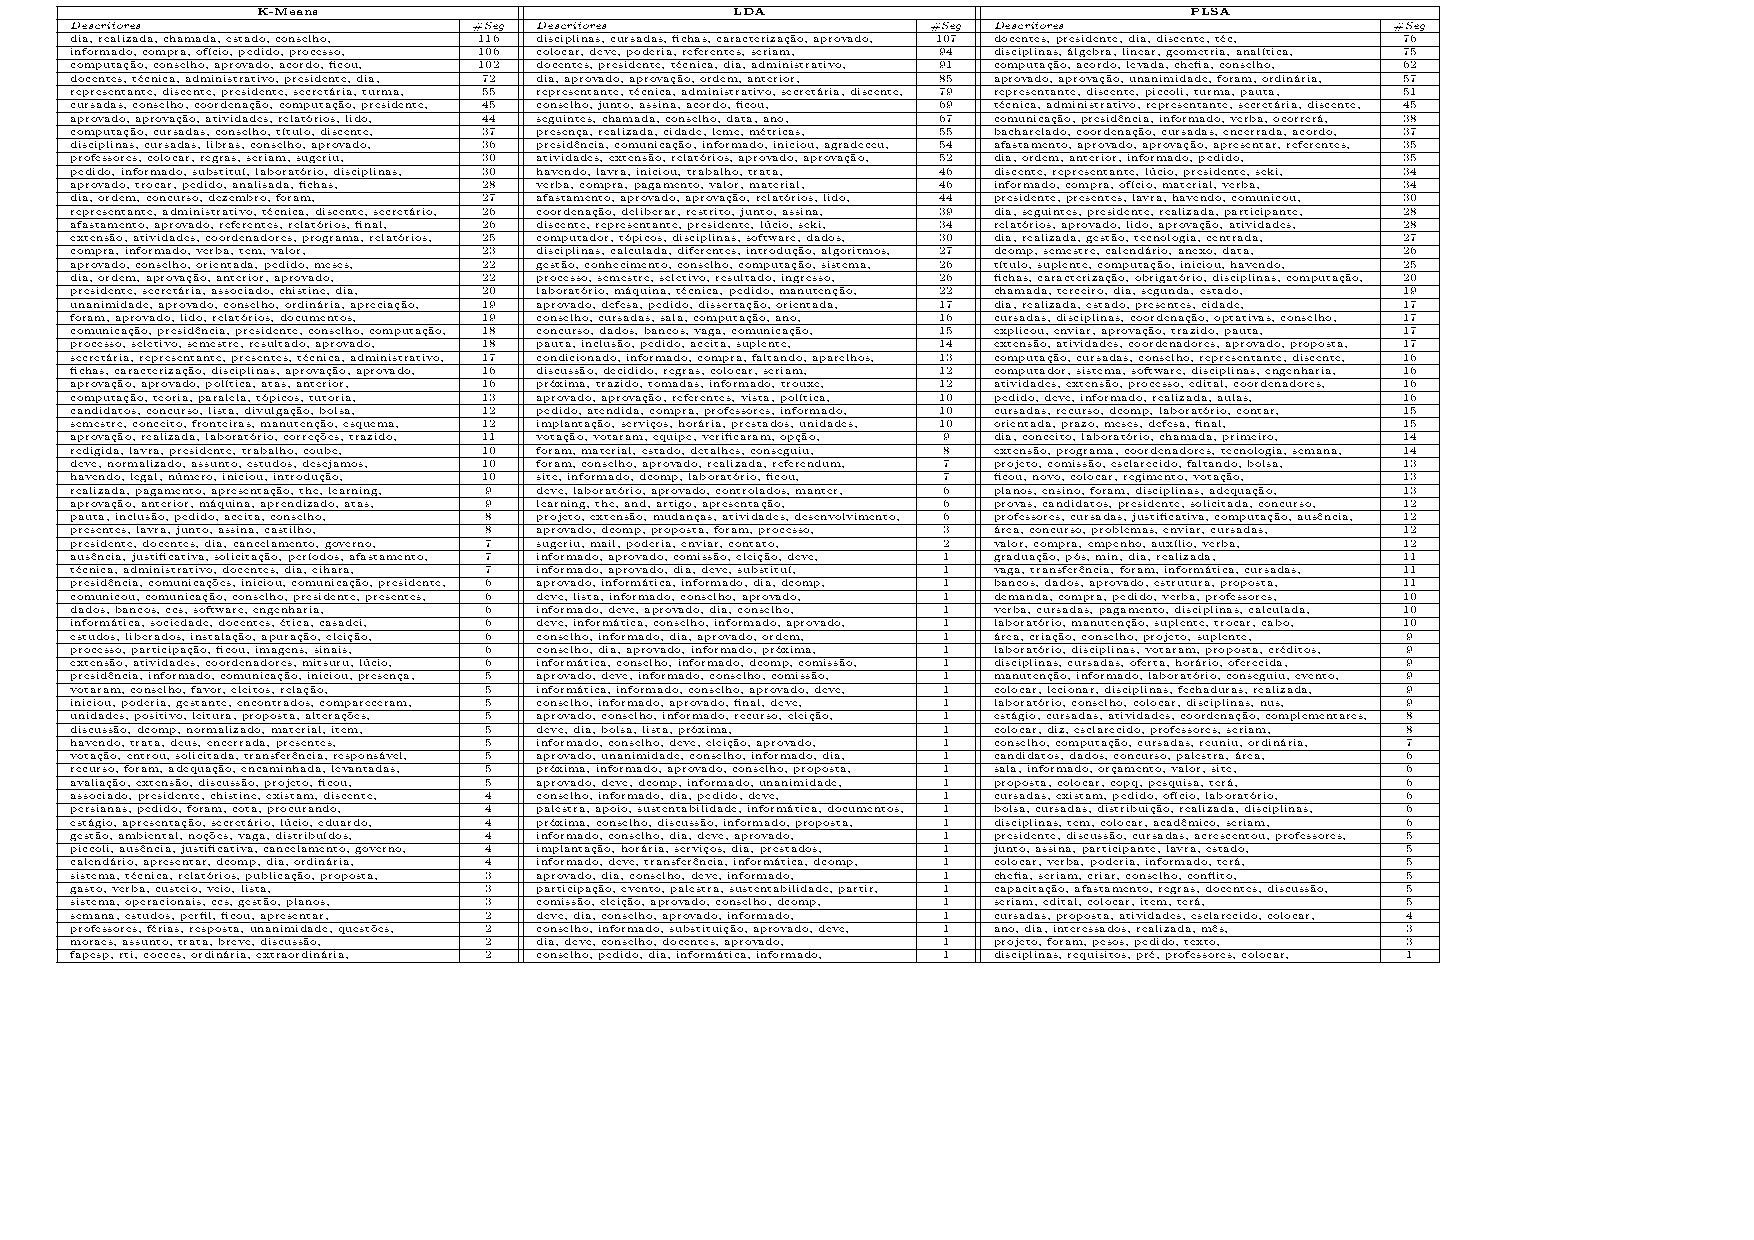
\includegraphics[trim={ 40 0 0 0 }, trim={ 0 60 0 66 }, page=1,width=1.1\textwidth]{anexos/tabelas/distribuicao-topicos/distribuicao-topicos.pdf}
	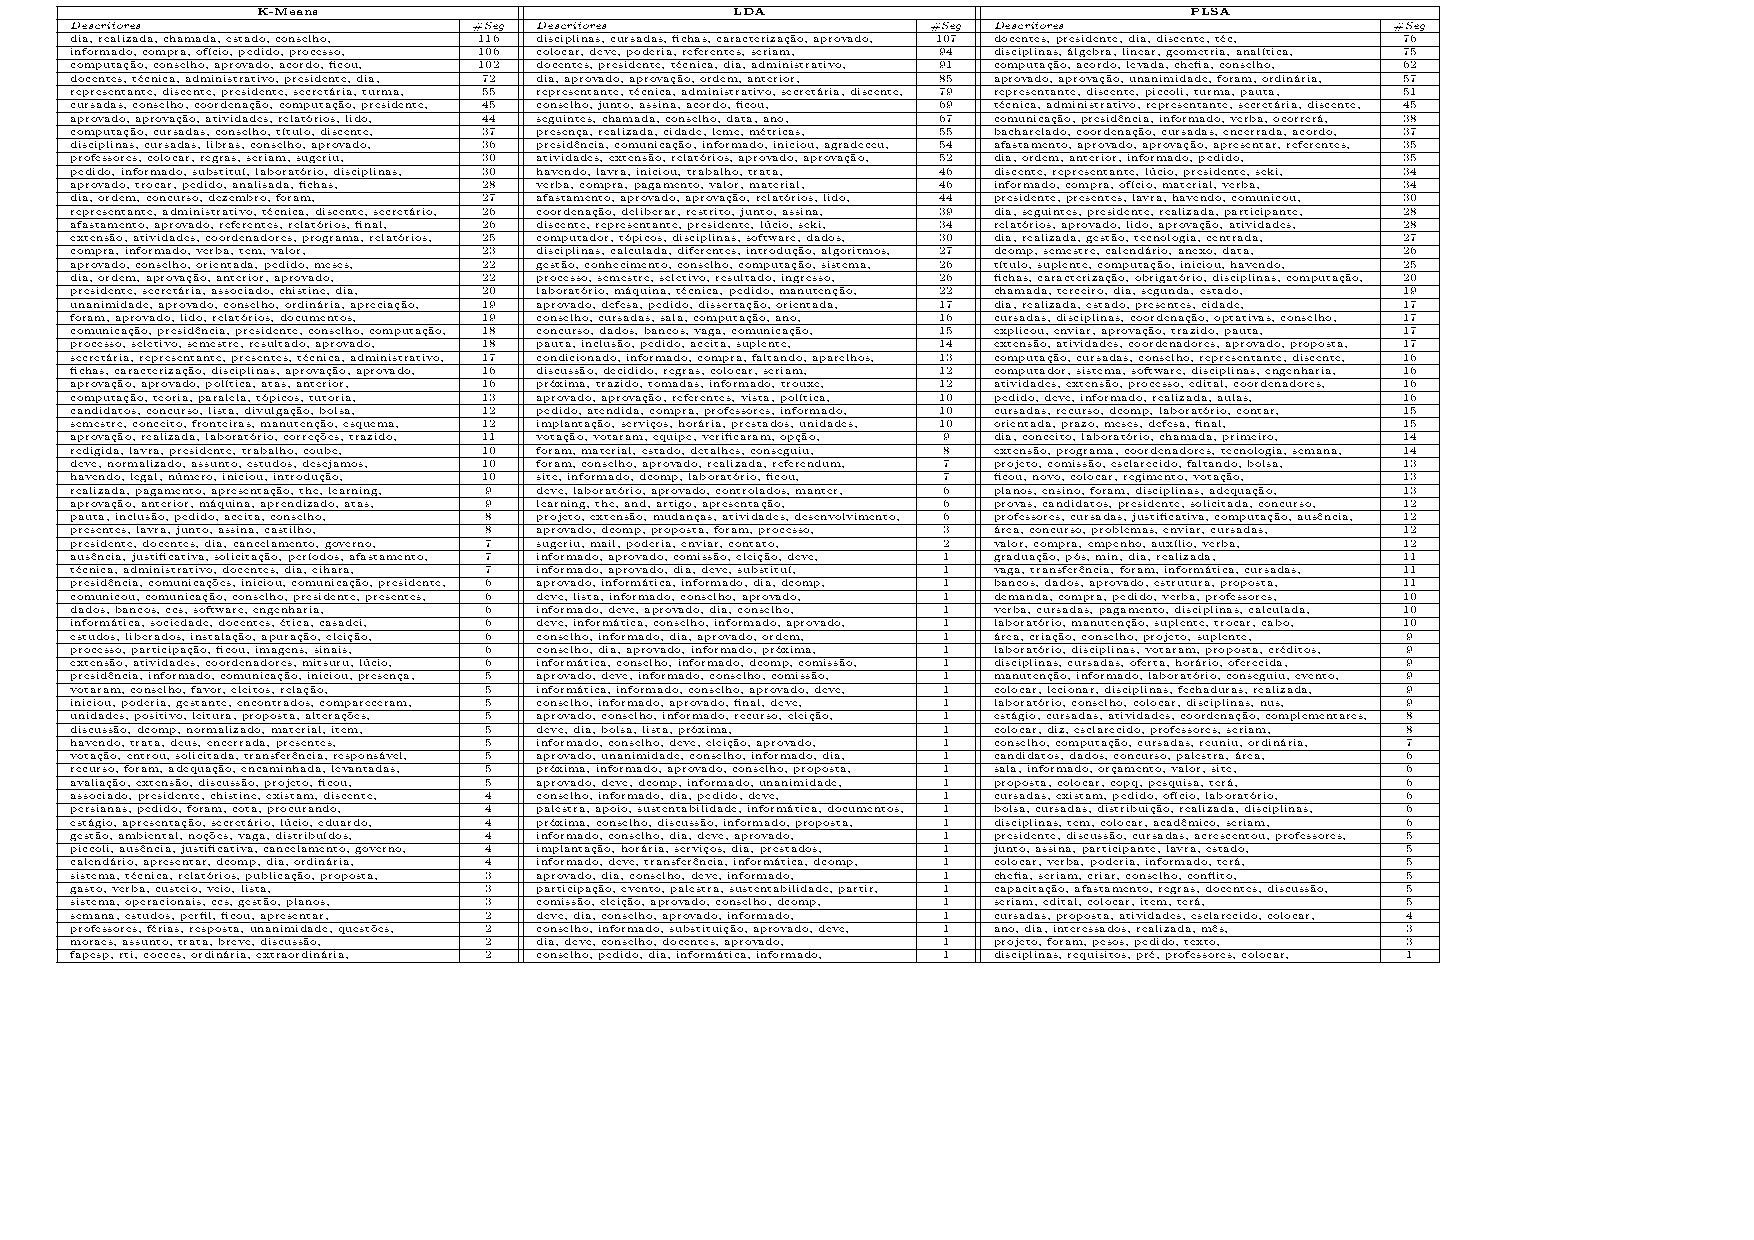
\includegraphics[trim={ 40 600 200 0 }, page=1,width=1.2\textwidth]{anexos/tabelas/distribuicao-topicos/distribuicao-topicos.pdf}
\end{figure}





\begin{table}[b]
	\caption{Distribuições dos tópicos obtidos pelos extratores.}
\end{table}




\end{landscape}

